\documentclass[11pt,a4paper]{article}
\usepackage[margin=1.45cm,top=1.2cm,bottom=1.25cm]{geometry}
\usepackage{amsmath,amssymb,mathtools}
\usepackage{xcolor}
\usepackage[normalem]{ulem}
\usepackage{tikz}
\usetikzlibrary{patterns}
\usepackage{enumitem}
\usepackage{array}
\usepackage{microtype}
\setlength{\parindent}{0pt}
\setlength{\parskip}{5pt}
\setlist[itemize]{leftmargin=1.1cm,itemsep=2pt,topsep=2pt}
\setlist[enumerate]{leftmargin=1.1cm,itemsep=2pt,topsep=2pt}
\allowdisplaybreaks

\definecolor{noteRed}{RGB}{225,20,20}
\definecolor{noteBlue}{RGB}{10,105,245}
\definecolor{noteGreen}{RGB}{0,125,80}
\definecolor{noteOrange}{RGB}{235,125,0}
\definecolor{notePurple}{RGB}{145,20,160}
\definecolor{board}{RGB}{236,242,231}
\newcommand{\rednote}[1]{\textcolor{noteRed}{#1}}
\newcommand{\bluenote}[1]{\textcolor{noteBlue}{#1}}
\newcommand{\greennote}[1]{\textcolor{noteGreen}{#1}}
\newcommand{\orangenote}[1]{\textcolor{noteOrange}{#1}}
\newcommand{\purplenote}[1]{\textcolor{notePurple}{#1}}
\newcommand{\boardnote}[1]{%
\begin{center}\fcolorbox{black}{board}{\begin{minipage}{0.96\linewidth}\small #1\end{minipage}}\end{center}}
\newcommand{\handbox}[1]{\begin{center}\fbox{\(\displaystyle #1\)}\end{center}}
\newcommand{\annot}[1]{\textcolor{noteRed}{\textit{#1}}}

\begin{document}
\pagestyle{empty}

% Source page 2
\begin{minipage}{0.47\linewidth}
\[
\mathcal{L}(\varphi,\partial_m\varphi,x)
 =\left|\frac{\partial x'}{\partial x}\right|
 \mathcal{L}(\varphi',\partial'_m\varphi',x')
\]
\vspace{-8pt}
\begin{center}\small\begin{tabular}{c}\underline{absolute value of the determinant}\\[-2pt]\underline{of the Jacobian matrix}\end{tabular}\end{center}
\end{minipage}\hfill
\begin{minipage}{0.49\linewidth}
\begin{center}\fbox{\textbf{INGREDIENTS}}\end{center}
\textcircled{1} \textit{Jacobian} \textbf{term}:\\[-2pt]
transformation of coordinates:
\[
x'{}^m=x^m+\delta x^m
\]
Hence,
\[
\frac{\partial x'{}^m}{\partial x^p}
=\frac{\partial x^m}{\partial x^p}
 +\frac{\partial\delta x^m}{\partial x^p}
=\underbrace{\delta^m_p}_{\delta_p}
 +\underbrace{\partial_p\delta x^m}_{\partial_p\,\delta x^m},
\qquad \partial_p=\frac{\partial}{\partial x^p}.
\]
\end{minipage}

\[
\frac{\partial x'{}^m}{\partial x^p}
=\delta^m_p+\partial_p\delta x^m
\qquad
\underbrace{\delta^m_p}_{\text{zeroth order}}
\quad
\underbrace{\partial_p\delta x^m}_{\text{1st order in ``$\delta x$''}}
\]
\[
\Longrightarrow\quad \text{Jacobian matrix has the structure }\;\mathbf{1}+\varepsilon
\qquad (\varepsilon\ll1).
\]
\[
\det(\mathbf{1}+\varepsilon)=\exp\!\left[\operatorname{Tr}\ln(\mathbf{1}+\varepsilon)\right]
\]
\[
\text{1st order}\ \simeq\ \exp[\operatorname{Tr}(\varepsilon)],
\qquad
\text{1st order}=1+\operatorname{Tr}(\varepsilon).
\]
\[
\therefore\quad
\det\!\left(\frac{\partial x'}{\partial x}\right)
=1+\partial_m\delta x^m
\qquad
\rednote{\text{Einstein summation convention (one repeated index)}}
\]

\[
\text{But since }\partial_m\delta x^m\text{ is a first order correction,}
\quad\text{then its absolute value is smaller than one}
\]
\[
\Longrightarrow\quad
\left|\det\!\left(\frac{\partial x'{}^m}{\partial x}\right)\right|
=\det\!\left(\frac{\partial x'{}^m}{\partial x}\right)
=1+\partial_m\delta x^m.
\]

\textcircled{2} \;\text{the }$\varphi'(x')$\text{ term}:\\
we follow that:
\[
\varphi'(x')=\varphi'(x+\delta x)\qquad\text{coordinate transformation.}
\]
\[
\begin{aligned}
\text{Expansion}\atop\text{at first order}
\qquad\Longrightarrow\qquad
\varphi'(x')
&=\underbrace{\varphi'(x)}_{\rednote{\text{second order in ``$\delta$''}}}+\sum_M
 \left(\frac{\partial\varphi'}{\partial x'{}^M}\right)_{x'=x}\delta x^M.
\end{aligned}
\]
\begin{flushright}
\bluenote{\fbox{The derivative can be approximated by a zeroth order term coming from another expansion}}\quad
\greennote{\textcircled{1}\ $\delta x^M$\ \text{1st order term in ``$\delta x$''}}
\end{flushright}

% Source page 3
\[
\text{But:}\qquad
\left(\frac{\partial\varphi'}{\partial x'{}^m}\right)
=\underbrace{\left(\frac{\partial\varphi}{\partial x^m}\right)}_{\rednote{\text{second order terms}}}
+\rednote{\text{1st order correction terms in ``$\delta$''}}.
\]
\[
\therefore\qquad
\varphi'(x')=\varphi'(x)+\sum_m(\partial_m\varphi)\,\delta x^m.
\]

\textit{Moreover:}
\begin{center}
\fcolorbox{noteRed}{white}{\begin{minipage}{0.96\linewidth}
$\ast\ast$\quad\textbf{Definition:} we introduce the variation of the fields $\delta\varphi(x)$
\textbf{AT THE SAME POINT} $x$ by:
\[
\delta\varphi(x)=\varphi'(x)-\varphi(x).
\]
\end{minipage}}
\end{center}
\[
\text{Finally:}\qquad
\boxed{\varphi'(x')=\varphi(x)+\delta\varphi(x)+(\partial_m\varphi)\,\delta x^m}.
\]

\textcircled{3} \;\text{the }$(\partial_m\varphi')(x')$\text{ term}:\\
\textit{Starting point:}
\[
\begin{aligned}
\frac{\partial\varphi'}{\partial x'{}^m}
&=\frac{\partial}{\partial x'{}^m}
 \left\{\varphi(x)+\delta\varphi(x)+(\partial_p\varphi)\delta x^p\right\}\\
&=\frac{\partial x^n}{\partial x'{}^m}\frac{\partial}{\partial x^n}
 \left\{\varphi(x)+\delta\varphi(x)+(\partial_p\varphi)\delta x^p\right\}\\
&=(\delta_m^n-\partial_m\delta x^n)\left\{
 \partial_n\varphi+\partial_n\delta\varphi
 +\partial_n\left[(\partial_p\varphi)\delta x^p\right]\right\}\\
&=(\delta_m^n-\partial_m\delta x^n)\left\{
 \partial_n\varphi+\partial_n\delta\varphi
 +(\partial_n\partial_p\varphi)\delta x^p
 +(\partial_p\varphi)(\partial_n\delta x^p)\right\}.
\end{aligned}
\]
\rednote{inverse of the Jacobian matrix:}
\[
\frac{\partial x'{}^m}{\partial x^n}=\delta_n^m+\partial_n\delta x^m,
\qquad
(\mathbf{1}+\varepsilon)^{-1}\simeq\mathbf{1}-\varepsilon
\qquad\Longrightarrow\qquad
\frac{\partial x^n}{\partial x'{}^m}=\delta_m^n-\partial_m\delta x^n.
\]
\[
\begin{aligned}
\frac{\partial\varphi'}{\partial x'{}^m}
&=(\delta_m^n-\partial_m\delta x^n)\left\{
\underbrace{\partial_n\varphi}_{0\text{th order}}
+\underbrace{\partial_n\delta\varphi}_{\text{second order}}
+\underbrace{(\partial_n\partial_p\varphi)\delta x^p}_{\text{first order}}
+(\partial_p\varphi)(\partial_n\delta x^p)\right\}\\
&=\partial_m\varphi+\partial_m\delta\varphi
+(\partial_m\partial_p\varphi)\delta x^p
+\greennote{(\partial_p\varphi)(\partial_m\delta x^p)}
-\rednote{(\partial_m\delta x^n)(\partial_n\varphi)}.
\end{aligned}
\]
\begin{flushright}
\greennote{\sout{the two coordinate terms cancel}}\qquad
\rednote{\text{-- }$(\partial_m\delta x^n)$\text{ contribution}}
\end{flushright}
\[
\boxed{\partial_m\varphi'=\partial_m\varphi+\partial_m\delta\varphi
+(\partial_m\partial_p\varphi)\delta x^p}.
\]

% Source page 4
\textcircled{4} \;\text{The }$\mathcal L(\varphi',\partial\varphi';x')$\text{ term}:\\[2pt]
\textit{the starting point is:}
\[
\begin{aligned}
&\mathcal L\Bigl(\underbrace{\varphi+\rednote{\delta\varphi+(\partial_m\varphi)\delta x^m}}_{\rednote{\varepsilon}},
\underbrace{\partial_m\varphi+\bluenote{\partial_m\delta\varphi+(\partial_m\partial_p\varphi)\delta x^p}}_{\bluenote{\text{1st order ``}\varepsilon\text{''}}},
\underbrace{x^m+\greennote{\delta x^m}}_{\greennote{\varepsilon\text{ term}}}\Bigr)\\
&\simeq \mathcal L(\varphi,\partial_m\varphi;x)
+\orangenote{\left(\delta\varphi+(\partial_m\varphi)\delta x^m\right)}\frac{\partial\mathcal L}{\partial\varphi}\\
&\quad+\purplenote{\left(\partial_m\delta\varphi+(\partial_m\partial_p\varphi)\delta x^p\right)}
 \frac{\partial\mathcal L}{\partial(\partial_m\varphi)}
+\textcolor{magenta}{\delta x^m}\frac{\partial\mathcal L}{\partial x^m}
+\text{second order terms}.
\end{aligned}
\]
\textit{However, the total derivative of the Lagrangian density reads:}
\[
\partial_p\mathcal L
=(\partial_p\varphi)\frac{\partial\mathcal L}{\partial\varphi}
+(\partial_p\partial_m\varphi)\frac{\partial\mathcal L}{\partial(\partial_m\varphi)}
+\frac{\partial\mathcal L}{\partial x^p}.
\]
\begin{center}\rednote{$p\to m\qquad m\to p$}\end{center}
\[
\begin{aligned}
\text{Then:}\qquad
\mathcal L(\varphi',\partial'\varphi';x')
&=\mathcal L(\varphi,\partial\varphi;x)
+\delta x^m\left[(\partial_m\varphi)\frac{\partial\mathcal L}{\partial\varphi}
+(\partial_p\partial_m\varphi)\frac{\partial\mathcal L}{\partial(\partial_p\varphi)}
+\frac{\partial\mathcal L}{\partial x^m}\right]\\
&\quad+\delta\varphi\frac{\partial\mathcal L}{\partial\varphi}
+(\partial_m\delta\varphi)\frac{\partial\mathcal L}{\partial(\partial_m\varphi)}.
\end{aligned}
\]

\textit{We have found:}
\[
\begin{aligned}
\mathcal L(\varphi',\partial'\varphi';x')
&=\mathcal L(\varphi,\partial\varphi;x)
+(\partial_m\mathcal L)\,\delta x^m
+\delta\varphi\frac{\partial\mathcal L}{\partial\varphi}
+(\partial_m\delta\varphi)\frac{\partial\mathcal L}{\partial(\partial_m\varphi)}.
\end{aligned}
\]
\begin{center}\rednote{$\partial_m\mathcal L$}\end{center}

\begin{center}\fcolorbox{noteRed}{white}{\textcolor{noteRed}{\large Symmetry Condition}}\end{center}
\[
\begin{aligned}
\mathcal L(\varphi,\partial\varphi;x)
&=\left|\frac{\partial x'}{\partial x}\right|\mathcal L(\varphi',\partial'\varphi';x')\\
&=(1+\partial_m\delta x^m)\left[\mathcal L(\varphi,\partial\varphi;x)
+(\partial_p\mathcal L)\delta x^p
+\delta\varphi\frac{\partial\mathcal L}{\partial\varphi}
+(\partial_p\delta\varphi)\frac{\partial\mathcal L}{\partial(\partial_p\varphi)}\right].
\end{aligned}
\]
\[
\begin{aligned}
\Longrightarrow\quad
\mathcal L
&+\delta\varphi\frac{\partial\mathcal L}{\partial\varphi}
+(\partial_p\delta\varphi)\frac{\partial\mathcal L}{\partial(\partial_p\varphi)}
+(\partial_p\mathcal L)\delta x^p
+(\partial_m\delta x^m)\mathcal L,
\end{aligned}
\]
\begin{flushright}
\bluenote{$(\partial_p\mathcal L)\delta x^p$ comes from ``$\delta x^p$''}\qquad
\bluenote{$(\partial_m\delta x^m)\mathcal L$ comes from ``$\partial_m\delta x^m$''}
\end{flushright}
\[
\boxed{\delta\mathcal L
=\delta\varphi\frac{\partial\mathcal L}{\partial\varphi}
+(\partial_p\delta\varphi)\frac{\partial\mathcal L}{\partial(\partial_p\varphi)}
+\partial_p(\mathcal L\,\delta x^p)}
\qquad \rednote{A=0}.
\]
\textit{But:}
\[
(\partial_p\delta\varphi)\frac{\partial\mathcal L}{\partial(\partial_p\varphi)}
=\partial_p\left[\delta\varphi\frac{\partial\mathcal L}{\partial(\partial_p\varphi)}\right]
-\delta\varphi\,\partial_p\frac{\partial\mathcal L}{\partial(\partial_p\varphi)}.
\]
\begin{center}\rednote{$u'v\qquad (uv)'\;-;uv'$}\end{center}

% Source page 5/6
\textit{Then:}
\[
\begin{aligned}
A={}&\delta\varphi\frac{\partial\mathcal L}{\partial\varphi}
-\delta\varphi\,\partial_p\frac{\partial\mathcal L}{\partial(\partial_p\varphi)}
+\partial_p\left(\delta\varphi\frac{\partial\mathcal L}{\partial(\partial_p\varphi)}\right)
+\partial_p(\mathcal L\,\delta x^p)=0.
\end{aligned}
\]
\[
\Longleftrightarrow\quad
\delta\varphi\left[\frac{\partial\mathcal L}{\partial\varphi}
-\partial_p\frac{\partial\mathcal L}{\partial(\partial_p\varphi)}\right]
=-\partial_p\left(\mathcal L\,\delta x^p
+\delta\varphi\frac{\partial\mathcal L}{\partial(\partial_p\varphi)}\right).
\]
\begin{flushright}
\rednote{\text{involves the coordinate transformations}}\qquad
\rednote{\text{involves the field modification at the same point}}
\end{flushright}

\textbf{\large $\bullet$ c) the Noether theorem:}

Using the same assumptions as before. Moreover, $\varphi(x)$ is a solution
of the equation of motion, so it satisfies
\[
\frac{\partial\mathcal L}{\partial\varphi}
-\partial_p\frac{\partial\mathcal L}{\partial(\partial_p\varphi)}=0
\]
\[
\Longrightarrow\qquad
\partial_p\left(\mathcal L\,\delta x^p
+\delta\varphi\frac{\partial\mathcal L}{\partial(\partial_p\varphi)}\right)=0.
\]
\textbf{Noether Theorem:} For any trajectory of a system having a symmetry,
there is a current $J^m$ which is conserved:
\[
\partial_mJ^m=0
\]
with
\[
J^m=\mathcal L\,\delta x^m
+\delta\varphi\frac{\partial\mathcal L}{\partial(\partial_m\varphi)}.
\]
\begin{center}\rednote{$J^m$: Noether current}\end{center}

% Source page 7
\textbf{\large Comments:}

\textcircled{1} \; properties of the $J^m$ components.
\[
\left|
\begin{array}{ll}
J^0 & \text{temporal component}\\
J^i & \text{spatial components},\quad i\in[1,D-1]
\end{array}
\right.
\]
\[
\boxed{\partial_0J^0+\partial_iJ^i=0}
\qquad\text{equation of conservation}
\qquad ``\partial_t\rho+\operatorname{div}\vec J=0''.
\]

\boardnote{
\textit{Def:} the charge $Q$ associated to the Noether current is:
\[
Q=\int_{\widetilde\Omega_{D-1}}d^{D-1}x\,J^0(x)
\qquad\text{integration over all of the space (NOT the time)}.
\]
$Q$ should in principal depend on time, however:
\[
\frac{dQ}{dt}=\int_{\widetilde\Omega_{D-1}}d^{D-1}x\,\left.\partial_0J^0\right|_{c=1}
=-\int_{\widetilde\Omega_{D-1}}d^{D-1}x\,\partial_iJ^i
=-\oint_{\partial\widetilde\Omega_{D-1}}J^i\,d\Sigma_i.
\]
\begin{flushright}
\textcolor{olive}{Ostrogradsky-Green theorem $\Rightarrow$ flux integral\\
over the boundary of $\widetilde\Omega_{D-1}$}
\end{flushright}
}

In physics, there are 2 possibilities:
\[
\textcircled{1}\quad \varphi\neq0\ \text{on a closed domain of space}
\]
\[
\Longrightarrow\quad\text{we can choose the boundary to make the integral vanish.}
\]
\begin{center}
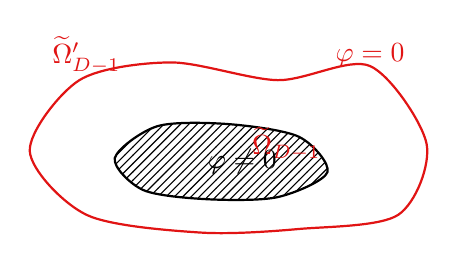
\begin{tikzpicture}[scale=0.9]
\draw[noteRed,thick] plot[smooth cycle] coordinates{(-3,0.1) (-2.3,1.1) (-1.0,1.35) (0.5,1.1) (1.8,1.3) (2.6,0.2) (2.2,-0.8) (0.8,-1.0) (-0.6,-1.05) (-2.2,-0.8)};
\fill[pattern=north east lines,pattern color=black] plot[smooth cycle] coordinates{(-1.8,0.0) (-1.2,0.45) (-0.2,0.48) (0.8,0.3) (1.2,-0.2) (0.5,-0.55) (-0.5,-0.58) (-1.4,-0.45)};
\draw[black,thick] plot[smooth cycle] coordinates{(-1.8,0.0) (-1.2,0.45) (-0.2,0.48) (0.8,0.3) (1.2,-0.2) (0.5,-0.55) (-0.5,-0.58) (-1.4,-0.45)};
\node[noteRed] at (-2.2,1.45) {$\widetilde\Omega'_{D-1}$};
\node[noteRed] at (0.62,0.20) {$\widetilde\Omega_{D-1}$};
\node[noteRed] at (1.8,1.45) {$\varphi=0$};
\node at (0,-0.05) {$\varphi\neq0$};
\end{tikzpicture}
\end{center}
\[
\int_{\Omega_{D-1}}\partial_iJ^i
=\int_{\widetilde\Omega_{D-1}}\partial_iJ^i.
\]

% Source page 8
\[
\textcircled{2}\quad \varphi\ \text{decreases ``fast enough'' at infinity so that}
\qquad \frac{\partial Q}{\partial t}=0
\qquad\Longrightarrow\qquad Q\ \text{is a constant}.
\]

\textcircled{2} \; Unicity of the Noether current:

The initial relation defines a structure for $J^m$.

But $J^m$ is defined from its divergence. So, show that:
\[
\widetilde J^M=J^M+\partial_NV^{NM}
\qquad\text{where}\qquad V^{NM}=-V^{MN}
\]
is also a Noether current (it satisfies the conservation law).

\textcircled{3} \; how to determine the Noether current: 2 ways
\[
\underline{1^{\mathrm{st}}}\ :\quad\text{use the expansion of }J^M
\]
\[
\underline{2^{\mathrm{nd}}}\ :\quad\text{compute }\;
\frac{\partial\mathcal L}{\partial\varphi}
-\partial_p\frac{\partial\mathcal L}{\partial(\partial_p\varphi)}
\quad\text{and see if it can be put into the form of a divergence term.}
\]

\end{document}
